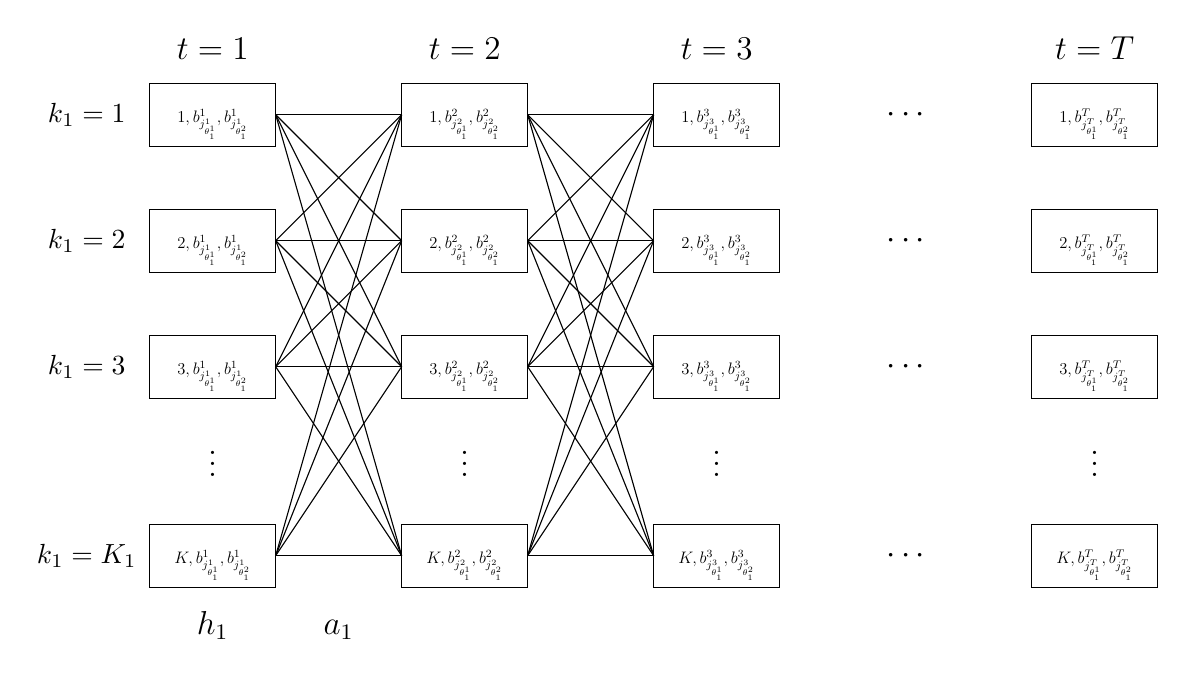
\begin{tikzpicture}[y=-1cm]

% objects at depth 50:
\draw[black] (3.8,4.2) -- (5.4,4.2);
\draw[black] (3.8,2.6) -- (5.4,2.6);
\draw[black] (3.8,5.8) -- (5.4,5.8);
\draw[black] (3.8,8.2) -- (5.4,8.2);
\draw[black] (3.8,2.6) -- (5.4,4.2);
\draw[black] (3.8,2.6) -- (5.4,5.8);
\draw[black] (3.8,2.6) -- (5.4,8.2);
\draw[black] (3.8,4.2) -- (5.4,2.6);
\draw[black] (3.8,4.2) -- (5.4,5.8);
\draw[black] (3.8,4.2) -- (5.4,8.2);
\draw[black] (3.8,5.8) -- (5.4,2.6);
\draw[black] (3.8,5.8) -- (5.4,4.2);
\draw[black] (3.8,5.8) -- (5.4,8.2);
\draw[black] (3.8,8.2) -- (5.4,2.6);
\draw[black] (3.8,8.2) -- (5.4,4.2);
\draw[black] (3.8,8.2) -- (5.4,5.8);
\draw[black] (7,4.2) -- (8.6,4.2);
\draw[black] (7,2.6) -- (8.6,2.6);
\draw[black] (7,5.8) -- (8.6,5.8);
\draw[black] (7,8.2) -- (8.6,8.2);
\draw[black] (7,2.6) -- (8.6,4.2);
\draw[black] (7,2.6) -- (8.6,5.8);
\draw[black] (7,2.6) -- (8.6,8.2);
\draw[black] (7,4.2) -- (8.6,2.6);
\draw[black] (7,4.2) -- (8.6,5.8);
\draw[black] (7,4.2) -- (8.6,8.2);
\draw[black] (7,5.8) -- (8.6,2.6);
\draw[black] (7,5.8) -- (8.6,4.2);
\draw[black] (7,5.8) -- (8.6,8.2);
\draw[black] (7,8.2) -- (8.6,2.6);
\draw[black] (7,8.2) -- (8.6,4.2);
\draw[black] (7,8.2) -- (8.6,5.8);
\draw[black] (5.4,2.2) rectangle (7,3);
\draw[black] (5.4,3.8) rectangle (7,4.6);
\draw[black] (5.4,5.4) rectangle (7,6.2);
\draw[black] (5.4,7.8) rectangle (7,8.6);
\path (6.2,7.2) node[text=black,anchor=base] {\large{}$\vdots$};
\draw[black] (8.6,2.2) rectangle (10.2,3);
\draw[black] (8.6,3.8) rectangle (10.2,4.6);
\draw[black] (8.6,5.4) rectangle (10.2,6.2);
\draw[black] (8.6,7.8) rectangle (10.2,8.6);
\path (9.4,7.2) node[text=black,anchor=base] {\large{}$\vdots$};
\draw[black] (2.2,2.2) rectangle (3.8,3);
\draw[black] (2.2,3.8) rectangle (3.8,4.6);
\draw[black] (2.2,5.4) rectangle (3.8,6.2);
\draw[black] (2.2,7.8) rectangle (3.8,8.6);
\path (3,7.2) node[text=black,anchor=base] {\large{}$\vdots$};
\draw[black] (13.4,2.2) rectangle (15,3);
\draw[black] (13.4,3.8) rectangle (15,4.6);
\draw[black] (13.4,5.4) rectangle (15,6.2);
\draw[black] (13.4,7.8) rectangle (15,8.6);
\path (14.2,7.2) node[text=black,anchor=base] {\large{}$\vdots$};
\path (3,1.9) node[text=black,anchor=base] {\large{}$t=1$};
\path (6.2,1.9) node[text=black,anchor=base] {\large{}$t=2$};
\path (9.4,1.9) node[text=black,anchor=base] {\large{}$t=3$};
\path (14.2,1.9) node[text=black,anchor=base] {\large{}$t=T$};
\path (1.4,2.7) node[text=black,anchor=base] {$k_1=1$};
\path (1.4,4.3) node[text=black,anchor=base] {$k_1=2$};
\path (1.4,8.3) node[text=black,anchor=base] {$k_1=K_1$};
\path (1.4,5.9) node[text=black,anchor=base] {$k_1=3$};
\path (3,9.2) node[text=black,anchor=base] {\large{}$h_1$};
\path (4.6,9.2) node[text=black,anchor=base] {\large{}$a_1$};
\path (11.8,2.7) node[text=black,anchor=base] {\large{}$\cdots$};
\path (11.8,4.3) node[text=black,anchor=base] {\large{}$\cdots$};
\path (11.8,5.9) node[text=black,anchor=base] {\large{}$\cdots$};
\path (11.8,8.3) node[text=black,anchor=base] {\large{}$\cdots$};
\path (3,2.7) node[text=black,anchor=base] {\large{}\scalebox{0.5}{$1,b^1_{j^1_{\theta^1_1}},b^1_{j^1_{\theta^2_1}}$}};
\path (3,4.3) node[text=black,anchor=base] {\large{}\scalebox{0.5}{$2,b^1_{j^1_{\theta^1_1}},b^1_{j^1_{\theta^2_1}}$}};
\path (3,5.9) node[text=black,anchor=base] {\large{}\scalebox{0.5}{$3,b^1_{j^1_{\theta^1_1}},b^1_{j^1_{\theta^2_1}}$}};
\path (3,8.3) node[text=black,anchor=base] {\large{}\scalebox{0.5}{$K,b^1_{j^1_{\theta^1_1}},b^1_{j^1_{\theta^2_1}}$}};
\path (6.2,2.7) node[text=black,anchor=base] {\large{}\scalebox{0.5}{$1,b^2_{j^2_{\theta^1_1}},b^2_{j^2_{\theta^2_1}}$}};
\path (6.2,4.3) node[text=black,anchor=base] {\large{}\scalebox{0.5}{$2,b^2_{j^2_{\theta^1_1}},b^2_{j^2_{\theta^2_1}}$}};
\path (6.2,5.9) node[text=black,anchor=base] {\large{}\scalebox{0.5}{$3,b^2_{j^2_{\theta^1_1}},b^2_{j^2_{\theta^2_1}}$}};
\path (6.2,8.3) node[text=black,anchor=base] {\large{}\scalebox{0.5}{$K,b^2_{j^2_{\theta^1_1}},b^2_{j^2_{\theta^2_1}}$}};
\path (9.4,2.7) node[text=black,anchor=base] {\large{}\scalebox{0.5}{$1,b^3_{j^3_{\theta^1_1}},b^3_{j^3_{\theta^2_1}}$}};
\path (9.4,4.3) node[text=black,anchor=base] {\large{}\scalebox{0.5}{$2,b^3_{j^3_{\theta^1_1}},b^3_{j^3_{\theta^2_1}}$}};
\path (9.4,5.9) node[text=black,anchor=base] {\large{}\scalebox{0.5}{$3,b^3_{j^3_{\theta^1_1}},b^3_{j^3_{\theta^2_1}}$}};
\path (9.4,8.3) node[text=black,anchor=base] {\large{}\scalebox{0.5}{$K,b^3_{j^3_{\theta^1_1}},b^3_{j^3_{\theta^2_1}}$}};
\path (14.2,2.7) node[text=black,anchor=base] {\large{}\scalebox{0.5}{$1,b^T_{j^T_{\theta^1_1}},b^T_{j^T_{\theta^2_1}}$}};
\path (14.2,4.3) node[text=black,anchor=base] {\large{}\scalebox{0.5}{$2,b^T_{j^T_{\theta^1_1}},b^T_{j^T_{\theta^2_1}}$}};
\path (14.2,5.9) node[text=black,anchor=base] {\large{}\scalebox{0.5}{$3,b^T_{j^T_{\theta^1_1}},b^T_{j^T_{\theta^2_1}}$}};
\path (14.2,8.3) node[text=black,anchor=base] {\large{}\scalebox{0.5}{$K,b^T_{j^T_{\theta^1_1}},b^T_{j^T_{\theta^2_1}}$}};

\end{tikzpicture}%
